% !TEX root = ../00_thesis.tex

% ------------------------------------------------------------------------------
% Global Positioning
In the previous chapter, we presented \baloo, a design framework for network stacks based on synchronous transmissions~(\ST).
The next two chapters of this dissertation focus on leveraging \ST for real-time applications.
In particular, we investigate the feasibility of providing end-to-end real-time guarantees in wireless cyber-physical systems (\CPS).

% ------------------------------------------------------------------------------
% Context
In \CPS, the communication among the sensing, actuating, and computing elements is often subject to hard real-time constraints.
In the embedded domain, real-time scheduling of dynamic applications has been extensively studied; real-time communication between wireless network interfaces is well studied as well.
Yet, the design of an entire system providing end-to-end real-time guarantees between distributed applications connected through a multi-hop wireless network remains an unsolved problem.


% ------------------------------------------------------------------------------
% What is the problem?
Indeed, providing end-to-end guarantees requires to jointly consider the scheduling of distributed applications \emph{and} the wireless communication protocol; whereas these are typically designed independently from each other, by people with different expertise.
Instead, we argue for a global design considering the complete message transmission chain: peripheral buses, memory accesses, networking interfaces, and the wireless communication protocol.

\begin{figure}
  \centering
  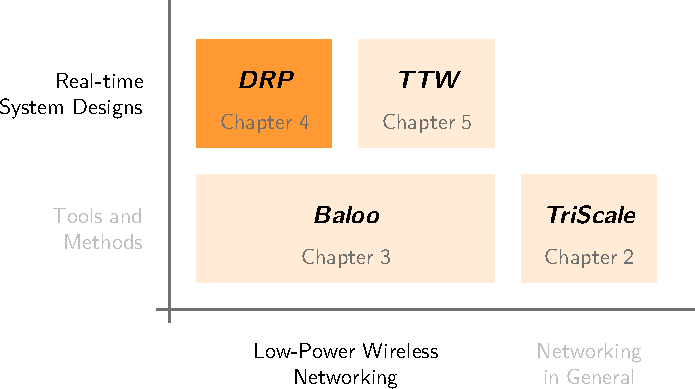
\includegraphics[scale=1]{chapter_drp}
  \caption{This chapter presents the Distributed Real-time Protocol (\DRP).
  \capt{\DRP provides end-to-end real-time guarantees using runtime contracts, aiming to maximize the flexibility of execution between distributed tasks.}}
  \label{fig:chapter_drp}
\end{figure}

% ------------------------------------------------------------------------------
% Claim
In this chapter, we propose to leverage the unique properties of \ST for designing reliable and efficient real-time wireless \CPS.
\ST abstracts the complexity of a multi-hop wireless network into a virtual ``wireless bus''~(\cref{ch:introduction}) which can then be scheduled similarly as a regular field bus.
Hence, traditional scheduling techniques can be applied to both the wireless network and the distributed applications, which facilitates designs of global real-time systems.

\pagebreak

\fakepar{Claim}
We demonstrate for the first time that end-to-end real-time guarantees can be obtained in low-power wireless networks by leveraging the efficiency and reliability of synchronous transmissions (\ST).
In particular, this chapter presents the Distributed Real-time Protocol (\DRP), a design using contracts to maximize the flexibility of execution between distributed tasks.

% ------------------------------------------------------------------------------
% Corresponding reference(s)
\begin{publi}

  The material from this chapter builds upon the work from Fabian Walter~\cite{walter2017Realtime} and Andreas Biri~\cite{biri2017Unleashing}. It relates to the following publication.

  \inlineRef%
  {End-to-End Real-Time Guarantees in Wireless Cyber-Physical Systems}%
  {Romain Jacob, Marco Zimmerling, Pengcheng Huang, Jan Beutel, Lothar Thiele}%
  {RTSS 2016. Porto, Portugal (December 2016)}

\end{publi}
